%!TEX root = ../Hardtung_PP_WiSe1920.tex

\section{Diagramming Notation}
\label{sec:conventions}


In order to define the concrete requirements of the planned diagramming program, all commonly used diagramming symbols and conventions have to be collected and categorized. After that groundwork a plan can be established on how to implement these findings in a desktop application.

The very fundamentals of Origami diagramming were developed and proposed by Akira Yoshizawa in his book \emph{Atarashi Origami Geijutsu (New Origami Art)}\cite{Yoshizawa} in 1954, which introduced a system of folding notation. Yoshizawas diagramming system is still widely used today and most commonly known as the  \emph{Yoshizawa–Randlett system}.

Despite its high popularity, different nuances and slight changes were made by different origami diagrammers.  To avoid further confusion, especially for beginners, american physicist and origami artist Robert J. Lang compiled notations that were in use by different folders and proposed a standard for all different folding sequences. In order to support his claims, Lang sent \enquote{a questionnaire to 25 diagrammers around the world}\cite{Lang} and tried to coherently argue in favour of, or against the various results.

Langs efforts were made under the assumption, that \enquote{[...] unless there is pressing reason otherwise, we should use the standard notation developed by Yoshizawa} \cite{Lang}.\\

To start off we have to define what exact components a diagram consists of. 
Most importantly, there always is a visual representation of the paper in the current step. This representation should show all or most (see Section \ref{sec:generalRules}) on when to leave out things creases, flaps, edges and layers to accurately show how the actual paper model would look like.
Secondly, there has to be a description of the actual folding sequence for one step. This description is comprised of a textual explanation and a visual display of the step with the diagramming symbols (Section \ref{sec:notation}). Both the verbal and the visual instructions should be able to stand for themselves, although that might not always be possible for complex steps. More detailed rules and specific terms for the verbal instructions are described on Section \ref{sec:generalRules}.

\subsection{General diagramming rules}
\label{sec:generalRules}

\begin{itemize}
	\item Be consistent (stick with one notation, e.g. -..-..-.. or -.-.-.-. for mountain folds)
	\item edges = 1 point line; creases 1/2 point line; creases should not contact the edges that the creases end upon; DO touch edges that they go under
	\item use right origami grammar
	\item show one white and one colored side of the paper
	\item distort the model to show all the layers
	\item enlarging the diagram with a circle or just by common sense with good diagrams
	\item right numbering of steps 1,2,3,4 and 1a,1b,1c to explain hard steps (ony to elaborate on a single step)
\end{itemize}

\newpage
\subsection{Diagramming Notation}
\label{sec:notation}

As there are quite a few simple and self-explanatory symbols, there will only be a further explanation if there are any additional rules or things to keep in mind while using them. Furthermore, on occasion Lang gives multiple valid symbols or ways to visualize a certain fold or folding sequence. The goal in these cases should be to give the user a choice on what method to use for a diagram. 

\subsubsection{Folds}
\label{sec:folds}

Starting with the very basics in origami, there has to be a differentiation between the types of folds. Generally, there are 2 different kinds, namely the \gls{valleyFold} and \gls{mountainFold}, which are shown in Figure \ref{fig:valleyFold} and Figure \ref{fig:mountainFold} respectively. Additionally the so called \gls{x-rayLine} is shown in Figure \ref{fig:x-rayLine}. Even though it is not a real fold, it was added here to show the three different forms a line can be drawn in origami diagrams. In order to indicate what kind of fold the X-Ray line is representing, you should extend the line past the paper and use a valley fold or mountain fold line.

\begin{figure*}[h]
    \centering
    \begin{subfigure}[b]{0.3\textwidth}
        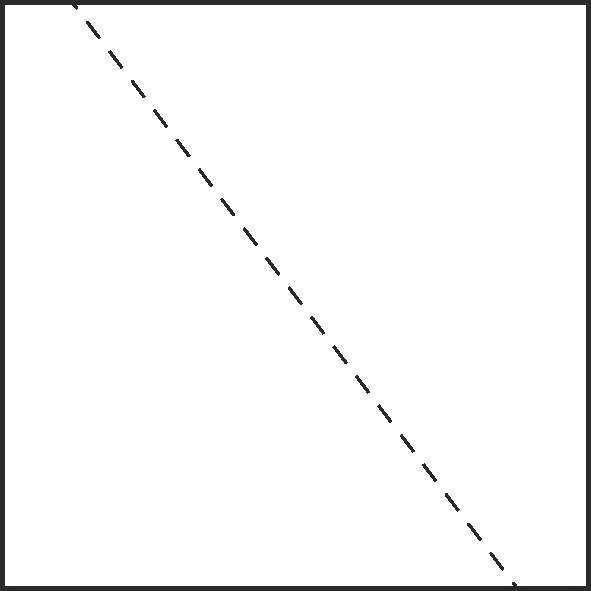
\includegraphics[width=\textwidth]{ValleyFold}
        \caption{Valley Fold}
        \label{fig:valleyFold}
    \end{subfigure}
    \begin{subfigure}[b]{0.3\textwidth}
        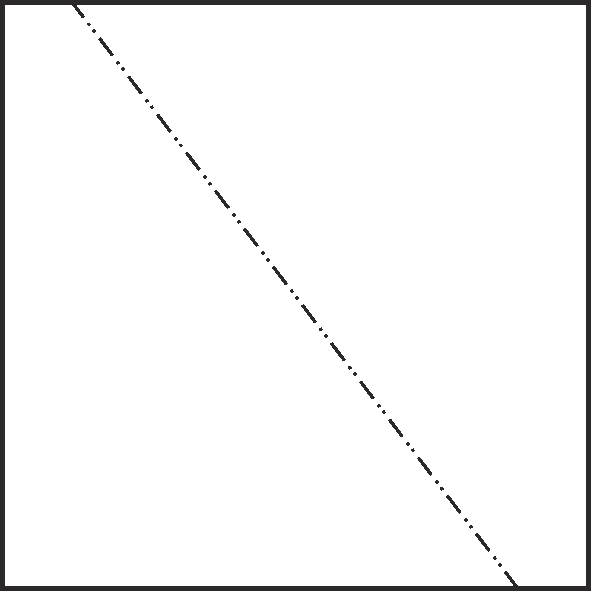
\includegraphics[width=\textwidth]{MountainFold}
        \caption{Mountain Fold}
        \label{fig:mountainFold}
    \end{subfigure}
    \begin{subfigure}[b]{0.3\textwidth}
        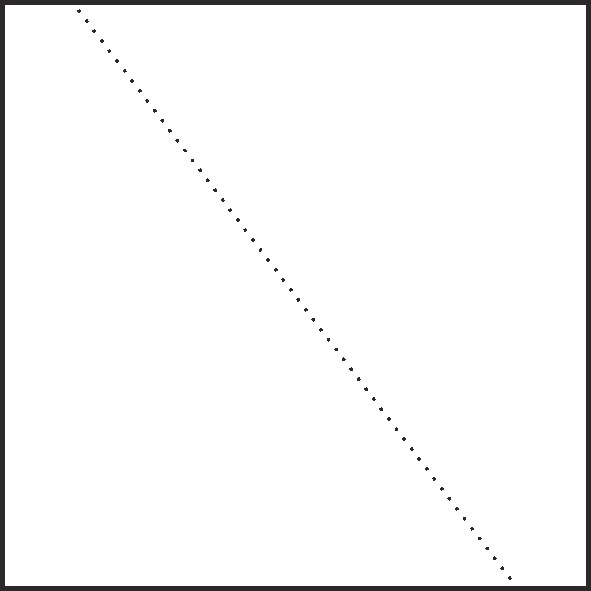
\includegraphics[width=\textwidth]{X-RayLine}
        \caption{X-Ray Line}
        \label{fig:x-rayLine}
    \end{subfigure}
    \caption{Different Lines in Origami Diagramming}\label{fig:origamiLines}
\end{figure*}

Important for the displaying of lines is, that they don't start or end with a gap. This method ensures that there isn't any ambiguity on what reference points are needed for the fold.


\subsubsection{Arrows}
\label{sec:arrows}

In order to show the folding steps unambiguously, there have to be arrows that indicate the direction the paper has to be folded. Showing only a valley or mountain fold leaves room for interpretation, which gets eliminated by the addition of these specific arrows. In origami diagramming there are two groups, the \gls{arrowsOfMotion} and \gls{arrowsOfAction}.
While the arrows of motion describe where the paper is folded to, the arrows of action indicate an action perfomed on the paper itself.

\begin{figure*}[h]
    \centering
    \begin{subfigure}[b]{0.3\textwidth}
        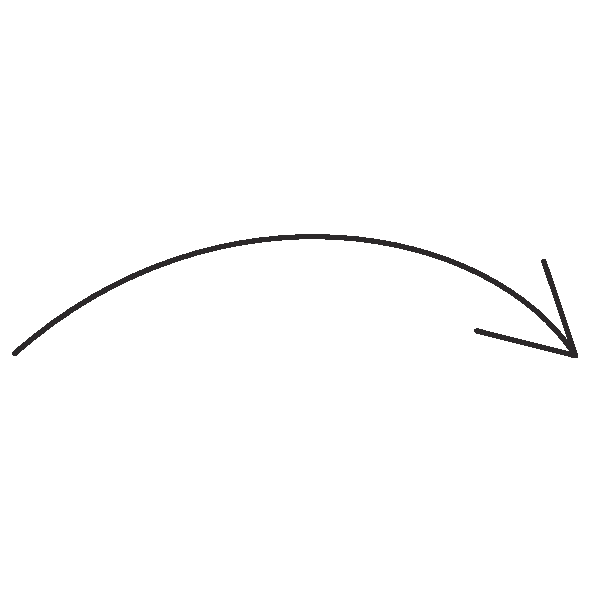
\includegraphics[width=\textwidth]{AoMValleyFold_thick}
        \caption{Valley Fold}
        \label{fig:aomValleyFold}
    \end{subfigure}
    \begin{subfigure}[b]{0.3\textwidth}
        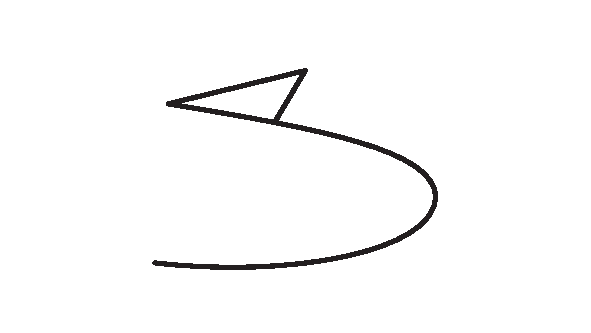
\includegraphics[width=\textwidth]{AoMMountainFold_thick}
        \caption{Mountain Fold}
        \label{fig:aomMountainFold}
    \end{subfigure}
    \begin{subfigure}[b]{0.3\textwidth}
        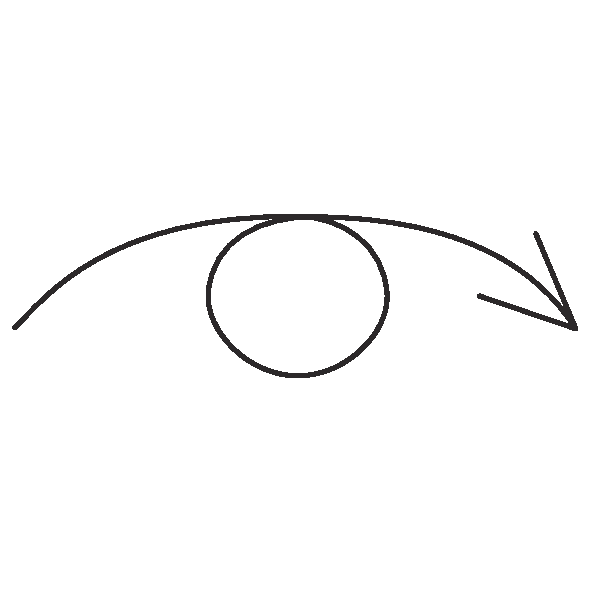
\includegraphics[width=\textwidth]{AoMTurnPaperOver_thick}
        \caption{Turn the paper over}
        \label{fig:aomTurnPaperOver}
    \end{subfigure}
    \caption{Arrows of Motion}
    \label{fig:arrowsOfMotion}
\end{figure*}
The unfolding arrow can either stand alone and signalize an unfolding action, or be combined with a valley/mountain fold and indicate a folding and unfolding procedure.
\begin{figure*}[h]
	\centering
	\begin{subfigure}[b]{0.4\textwidth}
		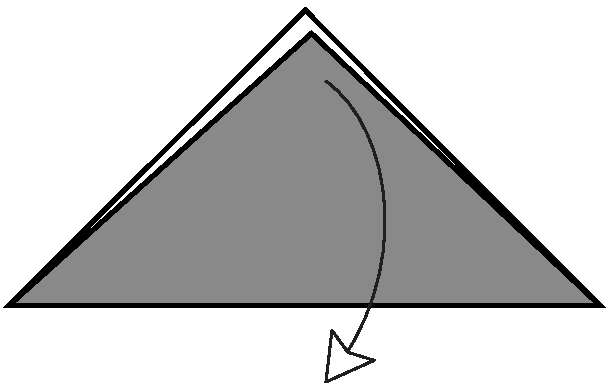
\includegraphics[width=\textwidth]{Unfold}
		\caption{Unfold}
		\label{fig:unfold}
	\end{subfigure}
	\begin{subfigure}[b]{0.3\textwidth}
		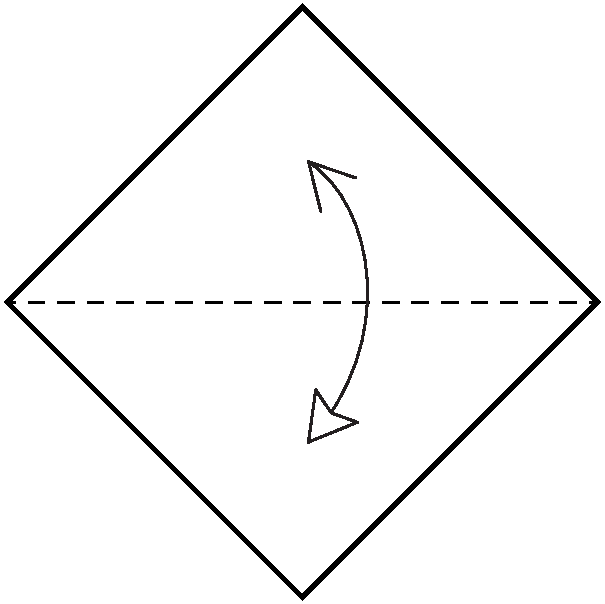
\includegraphics[width=\textwidth]{FoldAndUnfold}
		\caption{Fold and unfold}
		\label{fig:foldAndUnfold}
	\end{subfigure}
	\caption{Unfolding arrows}
	\label{fig:unfoldingArrows}
\end{figure*}
%
\begin{figure*}[h]
    \centering
    \begin{subfigure}[b]{0.3\textwidth}
        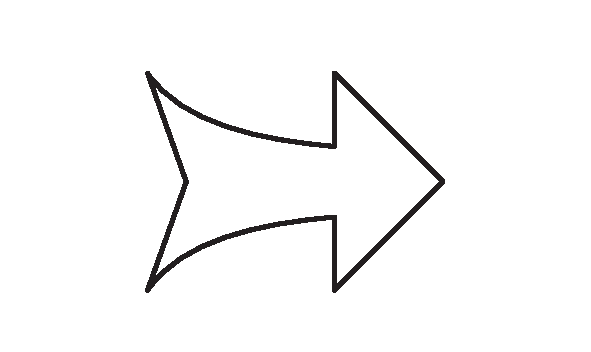
\includegraphics[width=\textwidth]{AoAPushHere_thick}
        \caption{Push here}
        \label{fig:aoaPushHere}
    \end{subfigure}
    \begin{subfigure}[b]{0.3\textwidth}
        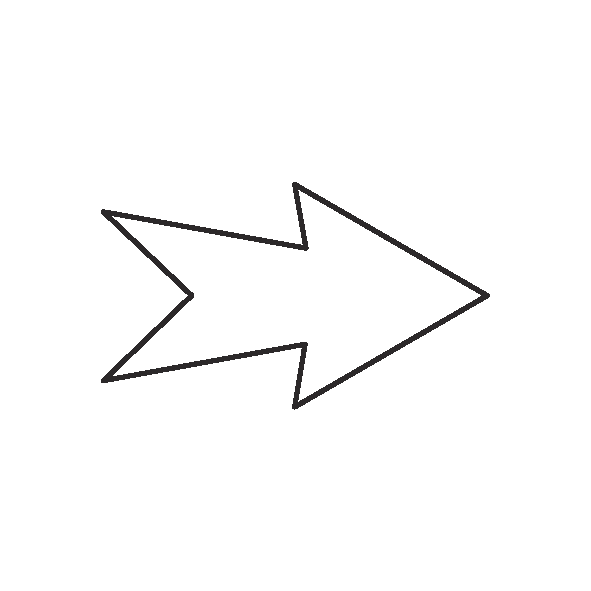
\includegraphics[width=\textwidth]{AoAPullPaperOut_thick}
        \caption{Pull the paper out}
        \label{fig:aoaPullPaperOut}
    \end{subfigure}
    \begin{subfigure}[b]{0.3\textwidth}
        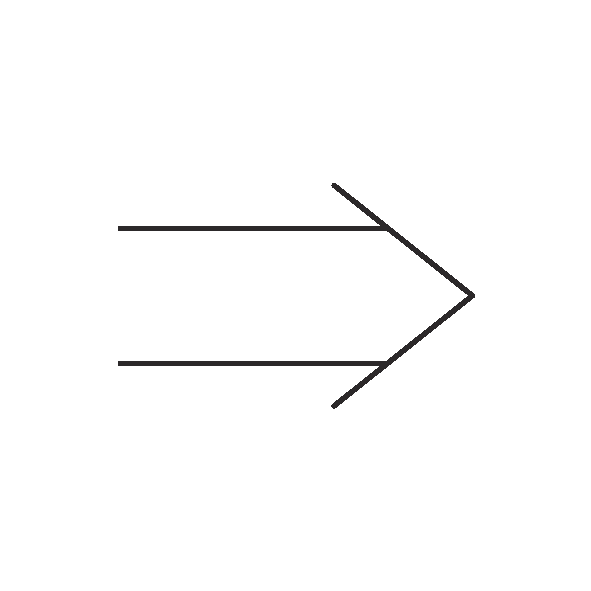
\includegraphics[width=\textwidth]{AoAInflateHere_thick}
        \caption{Inflate here}
        \label{fig:aoaInflateHere}
    \end{subfigure}
    \caption{Arrows of Action}
    \label{fig:arrowsOfAction}
\end{figure*}

\newpage

\subsubsection{Clarifying diagrams}

\textbf{Leader}
\begin{figure}[h]
	\centering
	\def\svgwidth{0.3\textwidth}
	\import{./images/}{Leader.pdf_tex}
	\caption{Use a leader to give additional information if needed}
	\label{fig:leader}
\end{figure}\\
%
\textbf{Equal distances}
\begin{figure}[h]
	\centering
	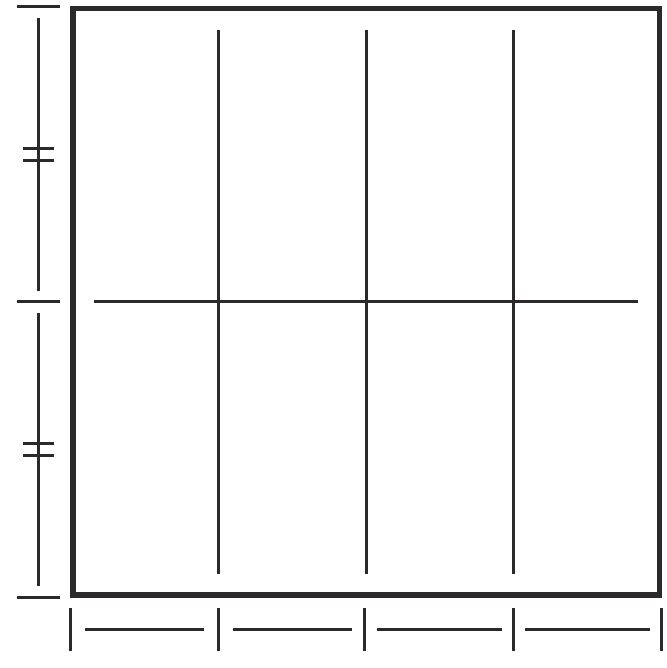
\includegraphics[width=0.3\textwidth]{EqualDistances}
	\caption{Equal Distances}
	\label{fig:equalDistances}
\end{figure}\\
%
\textbf{Equal angles}
\begin{figure}[h]
	\centering
	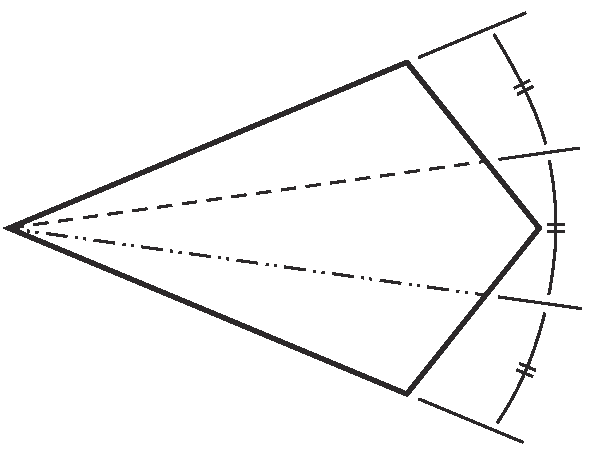
\includegraphics[width=0.3\textwidth]{EqualAngles}
	\caption{Equal Angles}
	\label{fig:equalAngles}
\end{figure}\\
%
\textbf{Rotations }
\begin{figure}[h]
	\centering
	\def\svgwidth{0.2\textwidth}
	\import{./images/}{Rotation.pdf_tex}
	\caption{Rotation Symbol}
	\label{fig:rotation}
\end{figure}\\
\newpage
%
\textbf{X-Ray View}
\begin{figure}[h]
	\centering
	\def\svgwidth{0.7\textwidth}
	\import{./images/}{X-RayView.pdf_tex}
	\caption{The X-Ray View shows hidden layers}
	\label{fig:x-rayView}
\end{figure}\\
%
\textbf{Repetitions }
\begin{figure}[h]
	\centering
	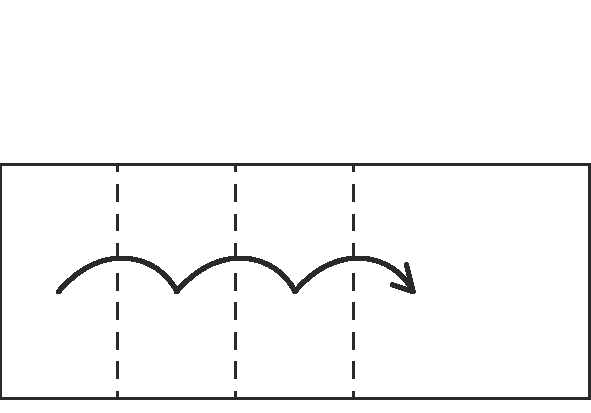
\includegraphics[width=0.6\textwidth]{FoldOverAndOver}
	\caption{Fold over and over}
	\label{fig:foldOverAndOver}
\end{figure}\\
For complicated repetitions you should show the result of the first fold that is to be repeated.
%
\begin{figure}[h]
	\centering
	\def\svgwidth{0.3\textwidth}
	\import{./images/}{RepeatBox.pdf_tex}
	\caption{Repetition Box}
	\label{fig:repeatBox}
\end{figure}\\
The repetition box from Figure \ref{fig:repeatBox} shows what exact steps are to be repeated and how many times.
\newpage
\textbf{Next view here}
\begin{figure}[h]
	\centering
	\def\svgwidth{0.6\textwidth}
	\import{./images/}{NextViewHere.pdf_tex}
	\caption{Next View Here}
	\label{fig:nextViewHere}
\end{figure}\\
%
\textbf{Hold here}
\begin{figure}[h]
	\centering
	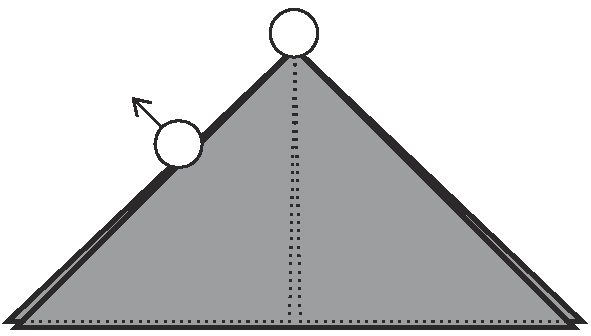
\includegraphics[width=0.6\textwidth]{HoldHere}
	\caption{Hold here + hold here and pull}
	\label{fig:holdHere}
\end{figure}\\

\newpage
\subsubsection{Folding Procedures}
\textbf{Rabbit Ear}\\
Lang gives two valid methods to visualize a \gls{rabbitEar}. While Figure \ref{fig:rabbitEarA} technically shows the more accurate format (according to the previously defined rules in Section \ref{sec:generalRules}), method B (see Figure \ref{fig:rabbitEarB}) is also desireable, as it shows the overall motion of the paper.
\begin{figure*}[h]
    \centering
    \begin{subfigure}[b]{0.4\textwidth}
        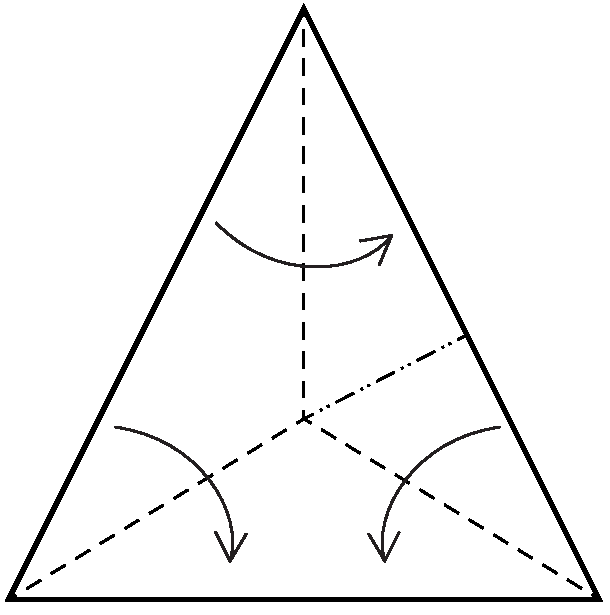
\includegraphics[width=\textwidth]{RabbitEarA}
        \caption{Rabbit Ear Method A}
        \label{fig:rabbitEarA}
    \end{subfigure}
    \begin{subfigure}[b]{0.52\textwidth}
        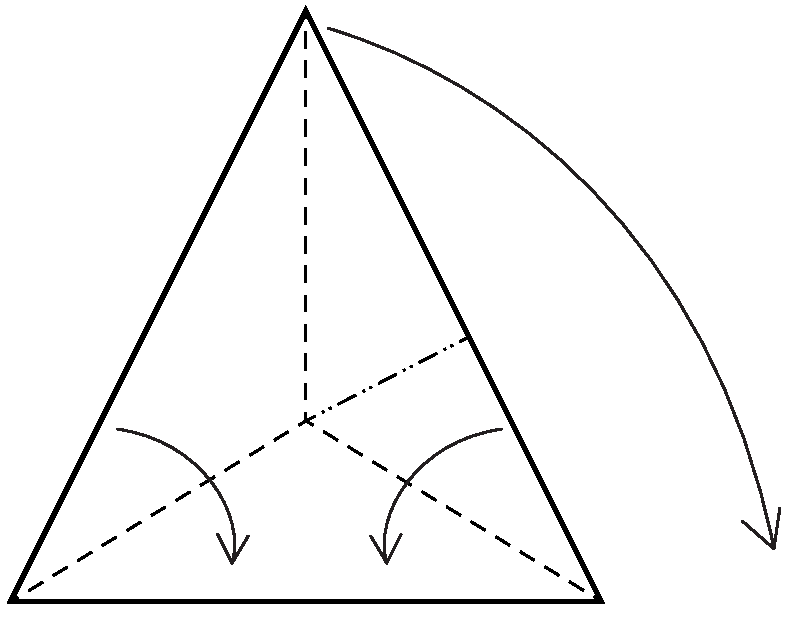
\includegraphics[width=\textwidth]{RabbitEarB}
        \caption{Rabbit Ear Method B}
        \label{fig:rabbitEarB}
    \end{subfigure}
    \caption{Both methods show a rabbit ear fold}
    \label{fig:rabbitEarMethods}
\end{figure*}
\begin{figure}[h]
	\centering
	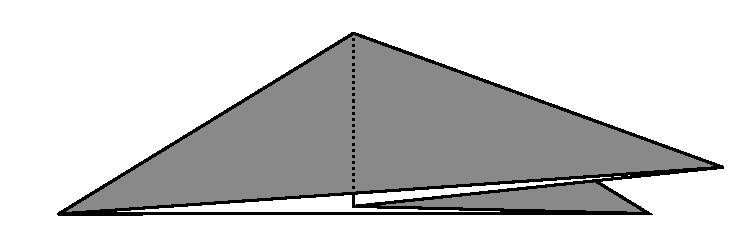
\includegraphics[width=0.8\textwidth]{RabbitEarResult}
	\caption{Rabbit Ear Result}
	\label{fig:rabbitEarResult}
\end{figure}\\
\newpage
\textbf{Reverse Folds}\\
Although Lang proposes two valid notations for outside reverse folds, for consistency's sake Method A should be used (see Figure \ref{fig:outsideReverseFoldA}).

\begin{figure*}[h]
	\centering
	\begin{subfigure}[b]{0.3\textwidth}
		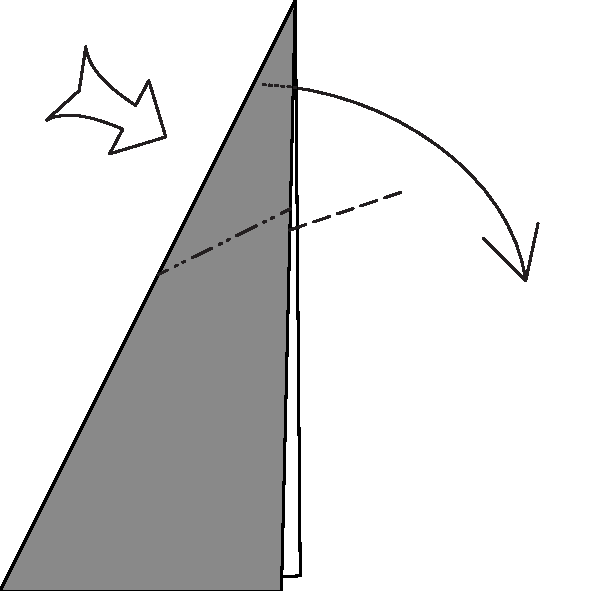
\includegraphics[width=\textwidth]{InsideReverseFold}
		\caption{Inside Reverse Fold}
		\label{fig:insideReverseFold}
	\end{subfigure}
	\begin{subfigure}[b]{0.3\textwidth}
		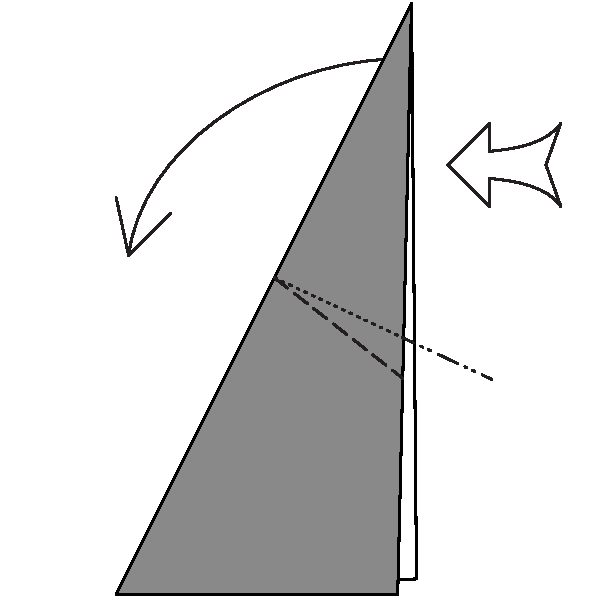
\includegraphics[width=\textwidth]{OutsideReverseFoldA}
		\caption{Outside Reverse Fold A}
		\label{fig:outsideReverseFoldA}
	\end{subfigure}
	\begin{subfigure}[b]{0.3\textwidth}
		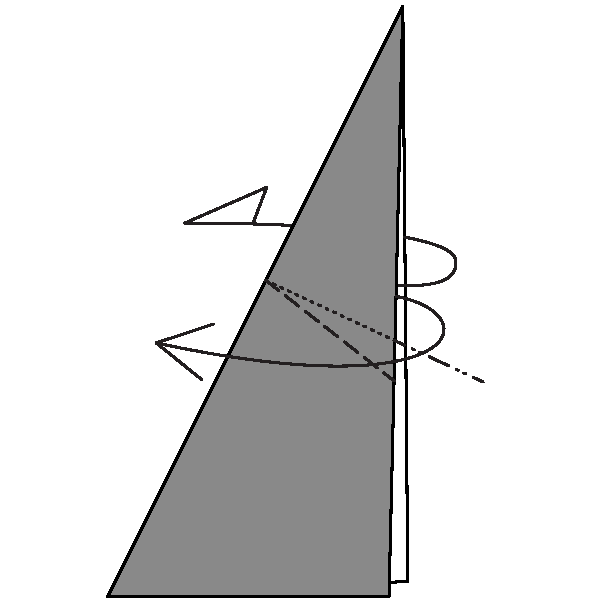
\includegraphics[width=\textwidth]{OutsideReverseFoldB}
		\caption{Outside Reverse Fold B}
		\label{fig:outsideReverseFoldB}
	\end{subfigure}
	\caption{Different reverse folds}
	\label{fig:reverseFoldMethods}
\end{figure*}

\textbf{Crimping and Pleating}\\
\begin{figure}[h]
	\centering
	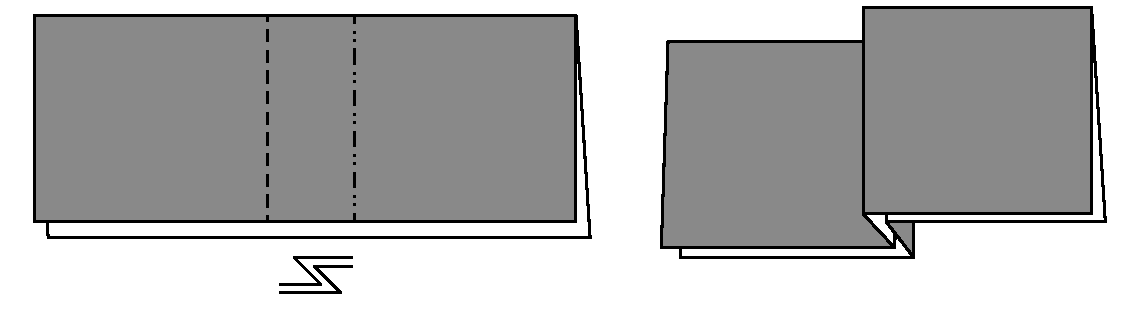
\includegraphics[width=0.8\textwidth]{Crimping}
	\caption{Crimping}
	\label{fig:crimping}
\end{figure}\\
\begin{figure}[h]
	\centering
	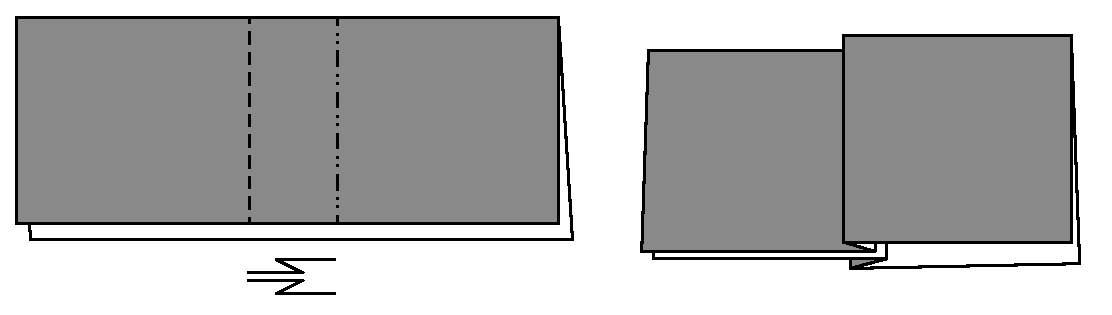
\includegraphics[width=0.8\textwidth]{Pleating}
	\caption{Pleating}
	\label{fig:pleating}
\end{figure}\\
\textbf{Sinks}
\begin{figure}[h]
	\centering
	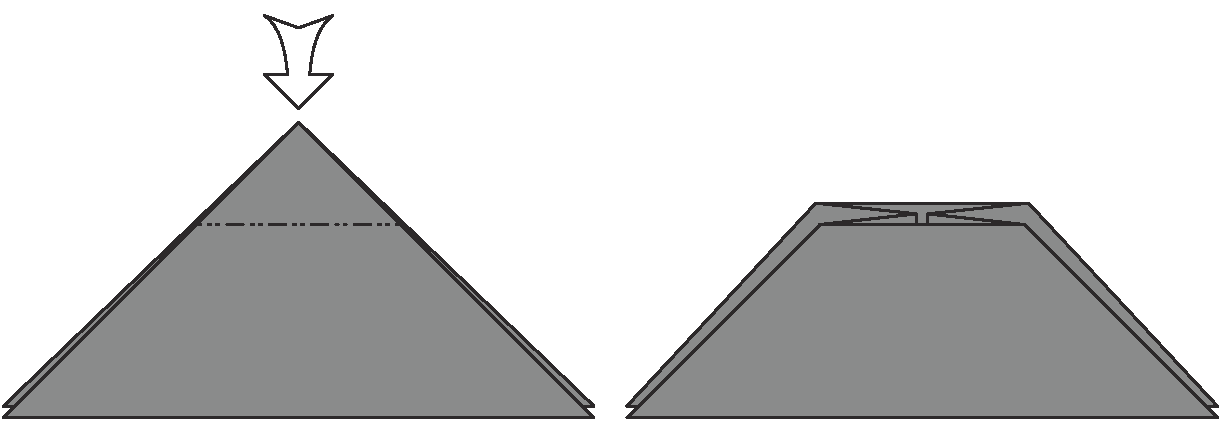
\includegraphics[width=0.8\textwidth]{OpenSink}
	\caption{Open Sink}
	\label{fig:openSink}
\end{figure}
\begin{figure}[h]
	\centering
	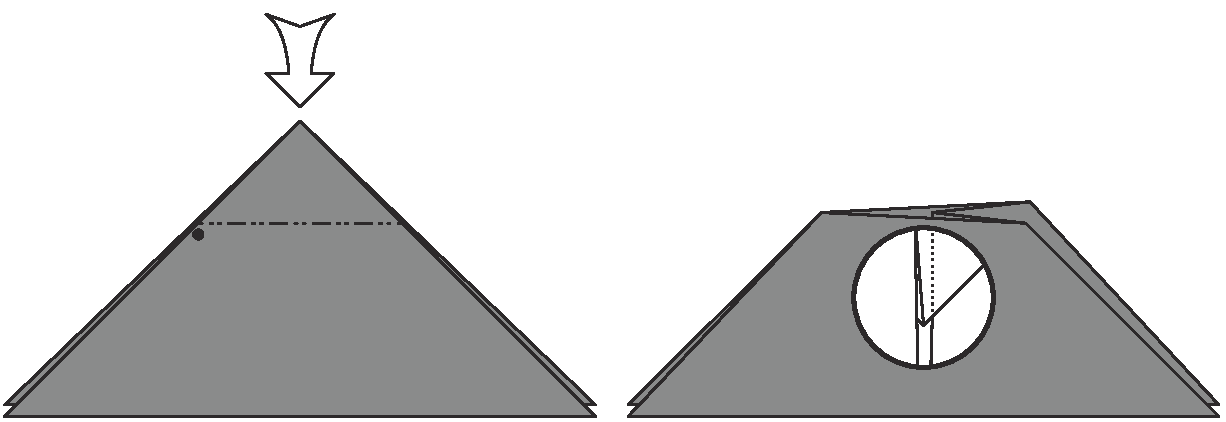
\includegraphics[width=0.8\textwidth]{MixedSink}
	\caption{Mixed Sink}
	\label{fig:mixedSink}
\end{figure}
\begin{figure}[h]
	\centering
	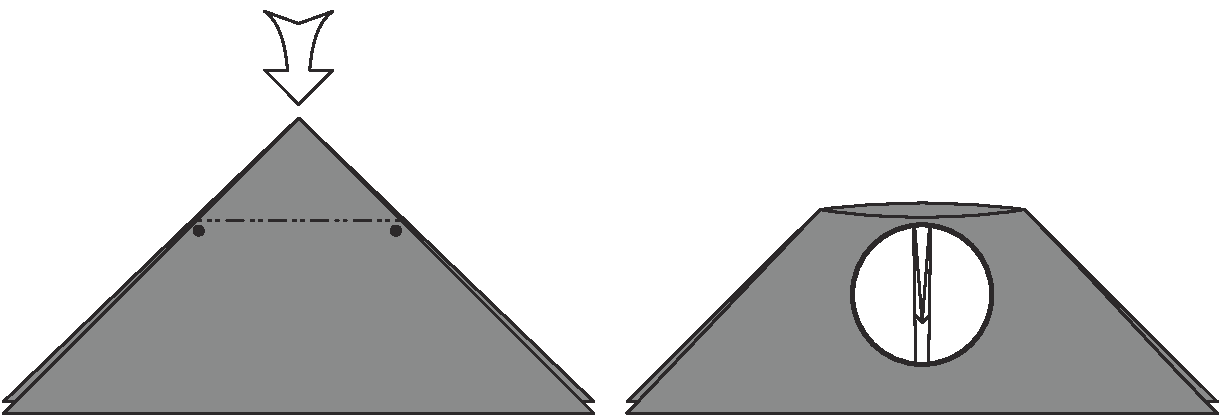
\includegraphics[width=0.8\textwidth]{ClosedSink}
	\caption{Closed Sink}
	\label{fig:closedSink}
\end{figure}










